\documentclass[11pt]{article}
\usepackage[margin=1.1in]{geometry}
\usepackage{amsmath,amssymb,amsthm}
\usepackage{booktabs}
\usepackage{array}
\usepackage{tabularx}
\usepackage[protrusion=true,expansion=false]{microtype}
\usepackage[table]{xcolor}
\usepackage{enumitem}
\usepackage{titlesec}
\usepackage{tikz}
\usepackage{float}
\usetikzlibrary{arrows.meta,positioning,calc}
\usepackage{hyperref}

\hypersetup{colorlinks=true, linkcolor=blue!60!black, urlcolor=blue!60!black, citecolor=blue!60!black}
\usepackage[skip=0.6\baselineskip, indent=0pt]{parskip}

\titleformat{\section}{\large\bfseries}{\thesection.}{0.7em}{}
\titleformat{\subsection}{\normalsize\bfseries}{\thesubsection.}{0.6em}{}

\newcommand{\vmax}{V_{\max}}
\newcommand{\Tc}{T_{\mathrm{close}}}
\newcommand{\tx}[1]{\texttt{#1}}
\newcolumntype{L}{>{\raggedright\arraybackslash}X}

\renewcommand{\arraystretch}{1.3}
\rowcolors{1}{}{black!5}

\definecolor{coop}{RGB}{232,245,233}
\definecolor{chainc}{RGB}{255,228,225}
\definecolor{hubc}{RGB}{255,243,214}

\title{\textbf{Lichen over BABE}\\withdrawals of a variable amount, by authenticated request\\[2pt]\large a design note with cost estimates}
\author{waxwing}
\date{Version 0.1, October 2026\\[2pt]\small a companion to \emph{Lichen}, version 0.2~\cite{lichen}}

\begin{document}
\maketitle

\begin{abstract}
BABE~\cite{babe} settles a Groth16 proof on Bitcoin in three
transactions, using witness encryption and a small garbled circuit, but
its statement, public inputs included, is fixed when the parties set up.
A lichen withdrawal is for an amount $b$ that Alice chooses only when she
withdraws. We describe how BABE can serve as lichen's on-chain gadget
without any change to its cryptography: the amount leaves the public
input and enters the witness, together with the hub's one-time signature
on it, which the hub must give on chain for exactly the amount Alice
asserted there, or lose. We sketch why this binds the proved amount to
the paid one, give the transaction graph, and estimate costs from BABE's
published measurements and lichen's: a refused withdrawal of about
31~kvB in six transactions against BitVMX's 100--212~kvB in 23--25, a
hub able to hold, for a dispute of a given length, about seven times as
many contracts before congesting the chain pays (three without
soldering), a
tower for Alice that holds none of her keys, since her only move due in
a window is a hash preimage, and a
setup per contract of about 14 minutes of computation with BABE's
soldering, or, we estimate, about 40 seconds with verifiable secret
sharing in its place, and 90--220~MiB of storage for the user. Nothing here is built, and the security argument is a
sketch.
\end{abstract}

\tableofcontents

\section{Status and scope}
\label{sec:status}

The main paper~\cite{lichen} treats the check of a disputed withdrawal
proof as a gadget with a narrow interface: given a proof whose public
input binds the program and its journal, adjudicate a two-party claim
on Bitcoin, with the contract's fixed terms checked, the amount $b$
readable by Script for a variable payout, and the loser paying. The
gadget built today is BitVMX's interactive search~\cite{bitvmx},
described and measured in a companion~\cite{lichenbitvmx}. This note
describes a second gadget, BABE, which is not built.

What is ours here is narrow: the binding of a late-chosen amount by the
hub's authentication (Section~\ref{sec:auth}), first put forward in a
discussion on Delving Bitcoin~\cite{delving}, and the cost estimates of
Section~\ref{sec:costs}. BABE, its witness encryption and its garbled
circuit are its authors'~\cite{babe,gkpw24,argo}; the problem of public
inputs that are known only at proving time has been treated at the
cryptographic layer by GOAT's researchers~\cite{goat}. Figures marked
(BABE) are the BABE paper's measurements, taken from its revised version
(October 2026), whose on-chain figures are larger than those of the
January version; figures marked (lichen) are measured in lichen's proof
of concept; the rest are our estimates.

\section{BABE in brief}
\label{sec:babe}

Groth16's verification, written additively in the target group, is
\[
  e(\pi_1, \pi_2) + e(\pi_3, \delta) = T, \qquad
  T = e(\alpha, \beta) + e(L, \gamma), \qquad
  L = \mathit{IC}_0 + \textstyle\sum_i s_i\, \mathit{IC}_i,
\]
where $\pi_1, \pi_2, \pi_3$ are the proof, $s_i$ the public inputs, and
the rest the verifying key. Witness encryption (WE) lets a party encrypt
a message so that only a holder of a valid proof can decrypt it. For
pairing relations \emph{linear} in the witness there is a simple
scheme~\cite{gkpw24}: for a secret scalar $r$, publish $r$ times the
public elements; a holder of the witness pairs it against them and
obtains $r\,T$, which unmasks the message. Groth16's check is not linear
in the witness, because of $e(\pi_1, \pi_2)$. BABE's idea is to supply
$r\pi_1$ by two-party computation once $\pi_1$ is known:
\begin{itemize}[leftmargin=1.5em]
\item \emph{Setup.} The verifier picks $r$ and a message $\mathit{msg}$,
  publishes the WE ciphertext ($r\delta$ and $\mathit{msg}$ masked by
  $r\,T$; 480~bytes), commits to $\mathit{msg}$ by its hash, and
  garbles a circuit computing $r\pi_1$ from the bits of $\pi_1$, with $r$
  inside. The circuit is small because group addition to a fixed point
  is linear in a six-term feature vector of the point, so all but a
  point-validation gadget is a decomposable randomized encoding with no
  garbled tables, after Argo MAC~\cite{argo}: 22~MiB per instance, 175~ms
  to make (BABE).
\item \emph{Assert.} The prover posts $\pi_1$ under a Lamport signature
  (508 bits).
\item \emph{ChallengeAssert.} To contest, the verifier must post the
  circuit's input labels for exactly those bits; a script checks that
  its labels and the prover's Lamport signature sign the same value. (A
  garbled circuit's input labels \emph{are} a Lamport signature of its
  input.)
\item The prover evaluates the circuit, obtains $r\pi_1$, completes the
  decryption with $\pi_2$ and $\pi_3$, and, if the proof is valid,
  publishes $\mathit{msg}$ (\emph{WronglyChallenged}), which blocks the
  verifier's \emph{Failure}; after a timelock $\Delta_2$ the prover's
  \emph{Success} pays. If the verifier never challenges, Success pays
  after $\Delta_2$ anyway. Failure needs $\Delta_1$ after the challenge,
  and $\Delta_2 > \Delta_1 + 2u$ for a liveness bound $u$.
\end{itemize}
On chain, a contested valid proof costs Assert 9,240~vB, ChallengeAssert
17,400~vB and WronglyChallenged 149~vB (BABE), with one set of labels.
Against a verifier who might garble wrongly (one whose circuit never lets
the prover decrypt), the prover checks the garbling by cut-and-choose:
for example 2,268 instances of which 4 are kept, 1~min~37~s and 1.8~GB at
peak on a 16-thread laptop (BABE). Without more, the verifier must then
post 4 sets of labels; \emph{soldering}, a SNARK proving the kept
instances' labels consistent, brings it back to one at about 12~minutes
more of setup (BABE); verifiable secret sharing could do the same in
seconds (Section~\ref{sec:vsss}). The WE is extractable, proved in the generic group
model, and the protocol is proved robust (an honest prover is paid) and
knowledge-sound (a prover who is paid knows a witness), for an honest
setup; cut-and-choose extends the setup to a malicious verifier.

\section{Where BABE fits in lichen}
\label{sec:fit}

\paragraph{The proving stack is unchanged.} lichen's withdrawal proof is
already a Groth16 proof over BN254: RISC Zero's recursion compresses the
guest's STARK receipts into a succinct receipt, and RISC Zero's
shrink-wrap proves that receipt's verification in Groth16, with RISC
Zero's single trusted setup~\cite{risc0}. BABE verifies exactly such a
proof. The guests, the STARKs, the sequencer's chain proofs and the
wrap all stay as they are; only the statement's journal changes
(Section~\ref{sec:auth}).

\paragraph{The roles.} Alice, who claims her withdrawal, is BABE's
prover; the hub, the only party a false claim can rob, is its verifier,
and so the garbler. BABE is a protocol between one prover and one
verifier, both known at setup, which is what a lichen contract is: no
committee, no open set of challengers, and no one else's funds in the
output. Designs whose challengers are not known in advance pay heavily
to approximate this; a bilateral contract has it for free.

\paragraph{Setup is per contract, and two-party.} The hub garbles for
each contract; Alice checks the garbling by cut-and-choose and keeps the
finalized instances. This replaces nothing in lichen's trust model: as
under BitVMX, the contract is set up by its two parties alone. What it
adds is cost at opening (Section~\ref{sec:setup}).

\paragraph{One-shot.} Revealing labels spends a garbled circuit's
security, so a BABE instance settles one claim. A lichen contract has at
most one withdrawal, after which it closes; renewal is a new contract
with a new setup.

\section{The fixed statement}
\label{sec:fixed}

BABE's ciphertext is built from $T$, and $T$ contains $e(L, \gamma)$,
the combination of the public inputs. So the whole public input is fixed
at setup. For a RISC Zero proof that input is the claim digest, a hash
over the image id and the journal; under BitVMX the journal is
$b \,\|\, c \,\|\, \mathcal{D}$, so setup would fix $b$, which Alice chooses only
when she withdraws. The ways round it that we know of:
\begin{itemize}[leftmargin=1.5em]
\item \emph{Supply $rL$ at proving time} for the asserted public input
  only, by envelopes opened with labels the verifier reveals per bit.
  With a single scalar public input this fails: the points
  $r\,2^j\mathit{IC}$ share one base, so one of them gives away
  $r\,\mathit{IC}$ and with it the ciphertext for any input. It needs
  each bit to be its own public input with an independent base, so a
  custom Groth16 wrap and its own trusted setup, and a garbled SHA-256
  between $b$ and RISC Zero's digest.
\item \emph{Deferred binding at the cryptographic layer}, as GOAT's
  researchers propose~\cite{goat}: a blinding point and further garbled
  circuits for the dynamic part of the input, one of them about 200
  million gates, and a larger challenge transaction.
\item \emph{One instance per digit value}: decompose $b$ in base $B$ and
  set up a fixed statement for each nonzero digit at each position. A
  dispute then proves each nonzero digit separately; base 16 for a
  14-bit amount means 60 setups per contract and up to four disputes.
\item \emph{Refresh the statement} whenever Alice's balance changes,
  which needs contracts in channels so that the refresh is off chain,
  and a setup per change of balance.
\item \emph{Set up only when withdrawing.} Rejected: a hub that declined
  the setup would leave Alice's tokens without collateral, which breaks
  the contract's first property, that within its cap Alice trusts the
  hub for nothing.
\end{itemize}

\section{Authenticated amounts}
\label{sec:auth}

\subsection{The statement}

Let the hub hold, per contract, a one-time signing key $pk_H$, fixed at
setup. The statement proved becomes
\[
  \exists\, b, w, \sigma_H:\quad
  \mathrm{Verify}(pk_H, b, \sigma_H) = 1 \;\wedge\;
  \mathrm{ValidWithdrawal}(c, \mathcal{D}, b, w) = 1,
\]
where $\mathrm{ValidWithdrawal}$ is lichen's withdrawal statement
unchanged (a return of $b$ to the hub with the contract's memo $c$, under
an anchored root of a valid history, with the contract's work on top)
and $w$ its witness. The journal holds only values fixed when the
contract opens: $c$, $\mathcal{D}$ and a digest of $pk_H$. The claim digest, and
so BABE's statement, is then fixed at setup, while $b$ is free until
Alice withdraws.

\subsection{The flow}

\begin{enumerate}[leftmargin=1.5em]
\item \emph{Request.} Alice asserts $b$ on chain under her one-time key
  for it, as she does today.
\item \emph{Response.} The hub must sign the same $b$ under $pk_H$, on
  chain, within its window. The response's script verifies both
  signatures and checks, digit by digit, that they sign the same value.
  If the hub is silent, Alice's timeout pays her the asserted $b$, as
  the hub's silence does under BitVMX.
\item \emph{Proof.} Alice proves the statement, using the hub's
  signature as part of her witness, and wraps the proof.
\item \emph{BABE.} Assert, ChallengeAssert, WronglyChallenged or
  Failure, as in Section~\ref{sec:babe}.
\item \emph{Payout.} Success pays through the bit outputs, which read
  $b$ from Alice's signature, as under BitVMX.
\end{enumerate}

\subsection{Why the amount is bound}
\label{sec:binding}

The hub's signature is not a judgement. It means ``this is the amount
being adjudicated'', not ``this withdrawal is valid'', and an honest hub
gives it mechanically for whatever Alice asserted, true or false. Three
links bind the amount proved to the amount paid:
\begin{itemize}[leftmargin=1.5em]
\item the proof's $b$ is the hub's, because the guest checks the hub's
  signature;
\item the hub's $b$ is Alice's on-chain $b$, because the response's
  script compares them digit by digit;
\item Alice's $b$ is the one paid, because the bit outputs read her
  signature, and a second signature from her under the same key forfeits
  them (\tx{equiv\_b}).
\end{itemize}
Suppose Alice asserts 100 but can prove a withdrawal of only 10. She has
the hub's signature on 100 and no valid withdrawal of 100, or a valid
withdrawal of 10 and no signature on 10. Neither satisfies the
statement.

\paragraph{The authenticator must be the hub.} Alice's own signature on
$b$ inside the witness would bind nothing: she could sign 10 privately
for the proof and 100 on chain for the payout, and the private
signature, hidden in a zero-knowledge witness, would never be seen, so
the equivocation could not be shown. A key she does not hold, used only
on chain, is what carries the on-chain value into a fixed statement. The
hub must therefore never sign a second value under $pk_H$, not even off
chain; its key is used once, in the response, and the cooperative fold
never touches it.

\paragraph{The payout could check both signatures.} Since the hub's
signature on $b$ is on chain, each bit output could require both
parties' signatures on the same value: Alice's leaf with bit $i$ set, the
hub's with it clear. Neither can then spend with a value the other did
not sign, which removes \tx{equiv\_b} and Alice's wait $\delta$ at about
the same script cost.

\subsection{The guest}

The withdrawal guest takes $b$ and $\sigma_H$ as private inputs, checks
$\sigma_H$ against $pk_H$, and commits $c$, $\mathcal{D}$ and $pk_H$'s digest. The
cost of the check depends on the signature's hash. LN-GAP's one-time
signatures chain \texttt{HASH160}, RIPEMD-160 of SHA-256: up to 150 chain
steps for a 32-bit word, and RIPEMD-160 has no accelerator in RISC
Zero's zkVM, so a few hundred thousand cycles, comparable to today's
whole statement of 389,000 (est.). Chains of SHA-256 instead, which
Script can check with \texttt{OP\_SHA256} at 32 bytes a chain value and
the zkVM accelerates, would cost a few thousand cycles (est.). The hub's
key should use them.

\subsection{Security, as a sketch}
\label{sec:security}

The statement is \emph{true} for any Alice holding any valid withdrawal:
for every amount, a hub signature on it exists mathematically. So
security cannot rest on the statement being false; it must rest on
extraction, that whoever is paid knows a witness, which then contains a
hub signature, which unforgeability then forces to be on the asserted
amount.

BABE gives the first step. Its knowledge soundness (Definition 9 of
\cite{babe}) states that for any NP relation, a prover who gets the
Success transaction onto the chain knows a witness, in the sense that an
extractor recovers one from its view. Here the relation is the
statement above, through two more layers: Groth16 is knowledge-sound
(in the generic or algebraic group model), so the Groth16 proof yields
a valid RISC Zero receipt; RISC Zero's STARKs are arguments of knowledge
(in the random-oracle model), so the receipt yields the guest's input,
$(b, w, \sigma_H)$. If $b \ne b^*$, the asserted amount, then $\sigma_H$
is a signature under $pk_H$ on a message the hub never signed, and the
hub signed exactly one: a forgery against a one-time signature.

What remains to be written properly:
\begin{itemize}[leftmargin=1.5em]
\item BABE's theorems are proved for an honest setup; the malicious-setup
  case rests on cut-and-choose, as for BABE itself.
\item The hub's signature arrives during the proving phase, after the
  statement is fixed, and depends on Alice's own assertion: the
  extraction must hold with the signature in the prover's view, which
  BABE's definition allows but which should be checked against its
  proof.
\item The composition of extractors across BABE, Groth16 and the STARKs,
  under BABE's restriction to benign auxiliary input.
\end{itemize}

\section{The transaction graph}
\label{sec:graph}

\begin{figure}[!htp]
\centering
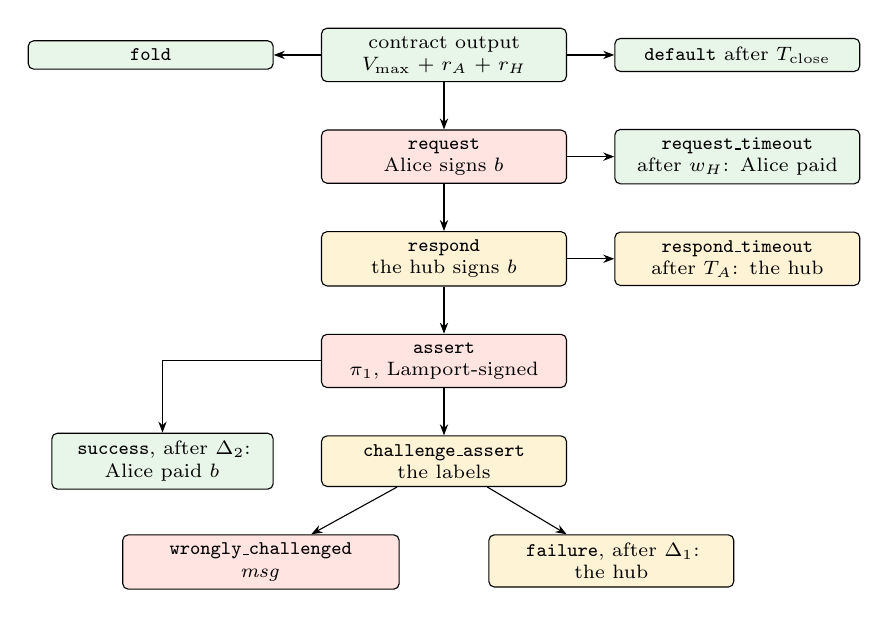
\begin{tikzpicture}[
  font=\scriptsize,
  tx/.style={draw, rounded corners=2pt, align=center, inner sep=3pt, text width=#1},
  tx/.default=29mm,
  >={Stealth[length=4pt]},
  node distance=6mm and 6mm,
]
\node[tx, fill=coop] (c) {contract output\\$\vmax + r_A + r_H$};
\node[tx, fill=coop, left=of c] (fold) {\tx{fold}};
\node[tx, fill=coop, right=of c] (def) {\tx{default} after $\Tc$};
\node[tx, fill=chainc, below=of c] (req) {\tx{request}\\Alice signs $b$};
\node[tx, fill=coop, right=of req] (rt) {\tx{request\_timeout}\\after $w_H$: Alice paid};
\node[tx, fill=hubc, below=of req] (resp) {\tx{respond}\\the hub signs $b$};
\node[tx, fill=hubc, right=of resp] (rspt) {\tx{respond\_timeout}\\after $T_A$: the hub};
\node[tx, fill=chainc, below=of resp] (as) {\tx{assert}\\$\pi_1$, Lamport-signed};
\node[tx, fill=hubc, below=of as] (ca) {\tx{challenge\_assert}\\the labels};
\node[tx, fill=coop, left=of ca, text width=26mm] (succ) {\tx{success}, after $\Delta_2$:\\Alice paid $b$};
\node[tx=33mm, fill=chainc, below left=6mm and -10mm of ca] (wc) {\tx{wrongly\_challenged}\\$\mathit{msg}$};
\node[tx, fill=hubc, below right=6mm and -10mm of ca] (fail) {\tx{failure}, after $\Delta_1$:\\the hub};
\draw[->] (c) -- (fold);
\draw[->] (c) -- (def);
\draw[->] (c) -- (req);
\draw[->] (req) -- (rt);
\draw[->] (req) -- (resp);
\draw[->] (resp) -- (rspt);
\draw[->] (resp) -- (as);
\draw[->] (as) -- (ca);
\draw[->] (as) -| (succ);
\draw[->] (ca) -- (wc);
\draw[->] (ca) -- (fail);
\end{tikzpicture}
\caption{The dispute's graph. Red: Alice's transactions; yellow: the
hub's; green: settlements. \tx{success} and \tx{failure} also spend the
value output of \tx{respond}; \tx{wrongly\_challenged} spends the output
\tx{failure} needs, so after it only \tx{success} remains.}
\label{fig:graph}
\end{figure}

The graph follows BABE's (its Appendix A.1), joined to lichen's contract
and payout (Figure~\ref{fig:graph}):
\begin{center}
\small
\begin{tabularx}{\linewidth}{>{\raggedright\arraybackslash}p{30mm}p{12mm}L}
\toprule
transaction & poster & spends, and what it carries or checks \\
\midrule
\tx{request} & Alice & the contract output; her one-time signature on $b$ (one word) \\
\tx{respond} & hub & \tx{request}'s output, within $w_H$; the hub's signature on $b$, and Alice's again for the digit-by-digit comparison; creates a value output and a connector \\
\tx{request\_timeout} & Alice & \tx{request}'s output after $w_H$; the payout, unverified \\
\tx{assert} & Alice & the connector, before an absolute deadline $T_A$; $\pi_1$ under her Lamport key \\
\tx{respond\_timeout} & hub & the value output and the connector, after $T_A$: Alice never asserted \\
\tx{challenge\_assert} & hub & \tx{assert}'s second output, within $\Delta_2 - \Delta_1$; the labels, matched to Alice's Lamport signature \\
\tx{wrongly\_challenged} & Alice & \tx{challenge\_assert}'s output, within $\Delta_1$; the preimage $\mathit{msg}$ \\
\tx{failure} & hub & the value output, \tx{assert}'s first output and \tx{challenge\_assert}'s, after $\Delta_1$; the hub takes everything \\
\tx{success} & Alice & the value output and \tx{assert}'s first output, after $\Delta_2$; the payout with its bit outputs \\
\bottomrule
\end{tabularx}
\end{center}
All but \tx{wrongly\_challenged} are pre-signed at opening, about nine
transactions. The payout and its bit outputs are as under BitVMX.

\paragraph{The assertion's deadline.} Alice's heavy move, \tx{assert},
needs no window: a late assertion only delays a payout the hub owes
anyway, and the hub loses nothing by waiting. So its deadline $T_A$ is
absolute, early enough before $\Tc$ that $\Delta_2$ and the payout fit,
and the proof, which needs the hub's signature first, never races a
timeout. What remains due within a window is, for Alice,
\tx{wrongly\_challenged} (149~vB) and, for the hub, its response and its
challenge.

\section{Alice's liveness: a keyless tower}
\label{sec:tower}

Under BitVMX, Alice cannot delegate her moves without her keys. Each move
signs, with a one-time key, hashes from her trace at positions the hub's
last choice selects, so it cannot be signed in advance; a tower that
plays her side holds her move keys, and by equivocating could lose her
the contract~\cite[\S 10]{lichenbitvmx}. Making those moves keyless would
need \texttt{OP\_CAT}. BABE removes the problem rather than shrinking
it: Alice's only commitments, $b$ and $\pi_1$, are fixed before anything
she must answer, and her one answer to the hub is a hash preimage, not a
signature. This is a difference of kind, not of count: a gadget with
fewer interactive moves would still need someone holding her keys while
the dispute runs; here no one does.

\paragraph{What she signs, and when.} Two one-time signatures: on $b$,
for \tx{request}, made when she returns $b$ on the L2; and on $\pi_1$,
the Lamport signature of \tx{assert}, made once she has the proof. The
proof needs the hub's signature on $b$, so the second comes after
\tx{respond}, but before the loose, absolute deadline $T_A$: a second
visit, not a race. A prover she does not trust with keys can make the
proof; she checks it (one Groth16 verification) and signs $\pi_1$.

\paragraph{What the tower holds.} The pre-signed transactions, the two
signed witnesses, the kept garbled instances (about 89~MiB) and the WE
ciphertext, and her proof, which reveals nothing of the witness. From
these and the chain it plays everything left to Alice:
\begin{itemize}[leftmargin=1.5em]
\item \tx{request\_timeout} and \tx{success}: pre-signed, released by
  their timelocks;
\item \tx{wrongly\_challenged}: it reads the hub's labels from
  \tx{challenge\_assert}, evaluates the garbled circuit to $r\pi_1$,
  decrypts with $\pi_2$ and $\pi_3$, and posts $\mathit{msg}$.
\end{itemize}
Her bit outputs wait $\delta$ for her own key, as under BitVMX, and
nothing races her for them.

\paragraph{Two changes to make.} First, in BABE, the leaf
\tx{wrongly\_challenged} spends checks the prover's signature as well as
the hashlock, $\mathsf{HashLock}(h_{\mathit{msg}}) \wedge
\mathsf{CheckSig}(pk_P)$, signed when posted (its Appendix~A.1). lichen
would drop the signature. The leaf exists only to spend the connector \tx{failure}
needs, so whoever posts $\mathit{msg}$, a tower or a stranger who copies
it from the mempool, does what Alice wants; the hub, who knows
$\mathit{msg}$ from the start, would only defeat its own challenge. The
tower builds the spend when it is needed, with a fee input of its own.
Second, fees. The terminals (\tx{request\_timeout}, \tx{success}) are signed
\texttt{ALL|ANYONECANPAY}, and their broadcaster adds a coin of its
own~\cite[\S 6]{lichenbitvmx}: keyless already. But the links
(\tx{request}, \tx{assert}) keep their ids and are bumped through an
anchor only their poster can spend, which lichen today locks to the key
that also sweeps her winnings. The anchors need a key of their own,
guarding nothing but 330~sats each, which she can hand the tower with
the witnesses; or she posts both links herself, since neither is due in
a window.

\paragraph{A compromised tower can only stay silent.} It holds no key,
so it cannot sign a wrong move or a second value. That matters here:
given her Lamport key, a tower that signed two values of $\pi_1$ would
let the hub combine their bits into a third, signed bit by bit, and
challenge with labels for it; she could not decrypt, and \tx{failure}
would take everything. So the tower is not trusted like her own machine,
as under BitVMX, but like a Lightning watchtower: several can run at
once, strangers to her and to each other, and any one suffices. Her
wallet, for its part, signs one $\pi_1$ only, and keeps the proof it
signed.

\section{Estimates}
\label{sec:costs}

\subsection{Transactions and disputes}

\begin{center}
\small
\begin{tabularx}{\linewidth}{>{\raggedright\arraybackslash}p{60mm}L}
\toprule
transaction & size \\
\midrule
\tx{request}: one signed word & ${\sim}0.4$~kvB (est., from lichen's measured ${\sim}250$~vB a word) \\
\tx{respond}: two signed words and the comparison & ${\sim}0.6$~kvB (est.) \\
\tx{assert} & 9.24~kvB (BABE) \\
\tx{challenge\_assert}, one label set (soldered) & 17.4~kvB (BABE) \\
\tx{challenge\_assert}, four label sets & ${\sim}42$~kvB (est.: one set is about $17.4 - 9.2 = 8.2$~kvB) \\
\tx{challenge\_assert}, one label set by adaptor signatures (VSSS) & ${\sim}26$~kvB (est., Section~\ref{sec:vsss}) \\
\tx{wrongly\_challenged} & 0.15~kvB (BABE); ${\sim}0.21$ with a fee input \\
a timeout, \tx{failure}, \tx{success} & ${\sim}0.3$--$0.8$~kvB (est.) \\
the payout and Alice's sweep of her bits & ${\sim}3$~kvB (lichen) \\
\bottomrule
\end{tabularx}
\end{center}

\begin{center}
\small
\begin{tabularx}{\linewidth}{>{\raggedright\arraybackslash}p{56mm}LL}
\toprule
exit & BABE (est.) & BitVMX~\cite{lichenbitvmx} \\
\midrule
the hub present: a fold & 0.3~kvB & 0.3~kvB \\
the hub gone & ${\sim}3.8$~kvB: request, its timeout, the payout & 23.1~kvB \\
the hub refuses a true claim to the end & ${\sim}31$~kvB in six transactions (${\sim}56$ unsoldered) & ${\sim}120$~kvB in 23 \\
the hub disproves a false claim & ${\sim}28$~kvB (${\sim}53$ unsoldered) & 100.4~kvB \\
the worst case & the same: there is no separate case for reads & 200--212~kvB, a read lie \\
Alice's transactions, those due in a window & 4 (request, assert, wrongly challenged, success), one & 13, twelve \\
keys Alice's tower must hold & none, but an anchor key (Section~\ref{sec:tower}) & her move and hop keys, and her input words' \\
pre-signed per contract & about 9 & 141 \\
\bottomrule
\end{tabularx}
\end{center}
Most of the gain against a vanished hub comes from not publishing the
proof's input words before the hub moves; BitVMX could recover much of
it by demanding them only from a hub that is present~\cite{lichenbitvmx}.

\subsection{Congestion}

The main paper's rule, $N s \le w \cdot 1\,\mathrm{MvB}$ for $N$
contracts whose move of $s$ bytes is due in a window of $w$ blocks, must
hold for every window. Comparing gadgets by one window would be unfair
to the one with fewer: a BitVMX dispute is twelve windowed moves on each
side, one after another, so a hub safe at a given window under BitVMX
asks for a dispute twelve windows long. The fair basis is the dispute's
length $T$ for a given $N$, with each window sized to its move:
$N \le T \cdot 1\,\mathrm{MvB} / \sum_i s_i$, summed over the defender's
windowed moves~\cite[\S 9]{lichenbitvmx}.
\begin{center}
\small
\begin{tabularx}{\linewidth}{>{\raggedright\arraybackslash}p{34mm}LLL}
\toprule
& BABE, Alice against a hostile hub & BABE, the hub against hostile users & BitVMX, the binding side \\
\midrule
windowed moves & \tx{wrongly\_challenged}, 0.21~kvB & the response 0.6 and \tx{challenge\_assert} 17.4 (42 unsoldered) & as built, Alice: twelve windows sized to her proof; with a window per move, the hub \\
$\sum_i s_i$ & 0.21~kvB & 18~kvB (43) & 302~kvB; 121~kvB \\
contracts safe with a dispute of a day & ${\sim}690{,}000$ & 8,000 (3,400) & 480; 1,190 \\
of a week & --- & 56,000 (23,700) & 3,300; 8,350 \\
the dispute for 60,000 contracts & 13 blocks & 7.5 days (18 days) & 126 days; 50 days \\
\bottomrule
\end{tabularx}
\end{center}
Hostile users bind under BABE. For a dispute of the same length, BABE
holds about 6.7 times as many contracts as BitVMX with a window per move
(2.8 unsoldered), and 17 times as many as BitVMX as built (7 unsoldered).
A hostile hub stops mattering, since Alice's only windowed move is
149~vB; were her assertion given a window rather than a deadline, her
sum would be 9.5~kvB, about 106,000 contracts for a week. The hub's
response, 0.6~kvB in $w_H$, is part of its sum: 60,000 contracts need
$w_H$ of at least 36 blocks. Chunking BitVMX's path into separate windows
would not change these figures, since it shrinks the path's largest move
but not its sum.

\subsection{Reserves and time}

A reserve must cover the other side's fees in a dispute it loses. Alice's
side is about 12.5~kvB (request, assertion, the preimage, her payout),
against about 117 under BitVMX, so the hub's reserve per user falls
about tenfold: about 125,000~sats at 10~sat/vB rather than 1.2 million,
and the contract suits balances of some tens of thousands of sats
rather than half a million. The hub's side is about 18~kvB (43
unsoldered). A hostile hub stretches a dispute to about
$w_H + \Delta_2$ blocks after Alice's assertion, about 170 blocks with
$w_H = 12$, $\Delta_2 = 156$, $\Delta_1 = 12$, against about 430 under
BitVMX with the windows the main paper uses; a vanished hub's users wait
$w_H$, as now.

\subsection{Setup per contract}
\label{sec:setup}

The new cost. At BABE's operating point (2,268 instances, 4 kept), on a
16-thread laptop (BABE):
\begin{center}
\small
\begin{tabularx}{\linewidth}{>{\raggedright\arraybackslash}p{60mm}L}
\toprule
item & per contract \\
\midrule
cut-and-choose, both roles & 1~min~37~s, 1.8~GB at peak \\
soldering, for one label set on chain & 745~s more, the hub's \\
what Alice stores & ${\sim}89$~MiB (4 instances of 22~MiB); perhaps ${\sim}2$~MiB with Duty-Free Bits' 45-fold smaller encoding~\cite{dutyfree}, unverified for this use \\
transferred from the hub to Alice & at least the kept instances, ${\sim}89$~MiB (est.) \\
a hub opening 10,000 contracts & ${\sim}270$ laptop-hours, ${\sim}2{,}300$ with soldering: parallel, and again at each renewal \\
\bottomrule
\end{tabularx}
\end{center}
Fewer instances trade setup for chain space: keeping 10 of 78 sets up in
6~s but, unsoldered, puts 10 label sets on chain. Nearly all of the
soldered setup's 14 minutes is the soldering, not the cut-and-choose.

\subsection{Setup by verifiable secret sharing}
\label{sec:vsss}

Fourteen minutes of computation per contract, paid again at every
renewal, is probably more than opening a contract can bear; forty
seconds is not. Glock~\cite{glock} replaces soldering with verifiable
secret sharing (VSSS), and BABE's authors have prototyped that layer for
BABE's 508 input bits (BABE, §9.4), without a transaction design. This
is the setup we would want, and what it needs on chain is sketched
below.

\paragraph{Why BABE keeps 4 of 2,268.} Cut-and-choose fails only if
every kept instance is bad and every opened one good, so the error is
$\binom{N}{M}^{-1}$, held to $2^{-40}$. Unsoldered, each kept instance
puts a label set on chain; soldered, the proof's time grows with $M$
(745, 866 and 969~s for 4, 5 and 6, BABE). Either way $M$ must be small,
and a small $M$ forces a large $N$.

\paragraph{Secret sharing reverses that.} The hub shares each input
label, for each bit and each value, across the $N$ instances, with
threshold $N - M + 1$, and publishes commitments to the polynomials
(Feldman's, over secp256k1). Alice checks the opened instances' shares
against them. At proving time one label per bit goes on chain, the
shared secret itself; with the $N - M$ opened shares, Alice
interpolates the labels of every kept instance. The value Alice did not
assert stays hidden, since only $N - M$ points of its polynomial are
known. The chain carries one label set whatever $M$ is, and the cost
moves to $N$, the shares to commit and check. So the right choice is
now a small $N$:
\begin{center}
\small
\begin{tabularx}{\linewidth}{>{\raggedright\arraybackslash}p{30mm}LL}
\toprule
$(N, M)$ & setup, both roles & Alice stores and receives \\
\midrule
(2,268, 4), soldered & ${\sim}14$~min (BABE) & ${\sim}89$~MiB \\
(78, 10), VSSS & ${\sim}40$~s (BABE's estimate: 33~s for the VSSS layer) & ${\sim}220$~MiB \\
(124, 8), VSSS & ${\sim}1$~min (54~s for the layer) & ${\sim}180$~MiB \\
(181, 7), VSSS & ${\sim}1.5$~min (84~s for the layer) & ${\sim}155$~MiB \\
\bottomrule
\end{tabularx}
\end{center}
That is about twenty times faster than soldering, and a hub opening
10,000 contracts spends about 110 laptop-hours rather than 2,300. The
bill moves to storage and transfer: Alice keeps every finalized instance,
22~MiB each, since she cannot know which one is honest. Glock's even
split, about 44 instances with 22 kept, would be the wrong end of that
trade here, at nearly 500~MiB. Duty-Free Bits' 45-fold smaller
encoding~\cite{dutyfree}, if it holds for these instances, would bring
even $M = 10$ to about 5~MiB.

\paragraph{On chain: adaptor signatures.} The label posted on chain
must be the secret Alice checked against the commitments, and the
chain must check that. A hashlock cannot: tying a hash to a committed
point $s G$ needs a proof, which is what soldering is. Glock uses
adaptor signatures instead. At setup Alice gives the hub, for each bit
$i$ and value $\beta$, a pre-signature on \tx{challenge\_assert} under
her own one-time key $A_{i,\beta}$, adapted to the committed label point.
The script selects $A_{i,\beta}$ by the bit of her Lamport signature, and
the hub can satisfy it only by completing her pre-signature, which
hands her the label. In Glock the garbler is also the prover, so its
adaptor signatures are its assertion; in BABE the prover asserts and the
verifier reveals, so both are paid for. Per bit that is a 64-byte
signature and two 32-byte keys in the leaf, about 135~bytes of witness
against about 65 for a hashed label, so \tx{challenge\_assert} grows to
about 9.2 + 17 $\approx$ 26~kvB (est.), against 17.4 soldered and about
91 for ten label sets unsoldered. Against hostile users, the hub's
windowed sum becomes about 27~kvB: about 37,000 contracts for a week's
dispute, against 56,000 soldered (Section~\ref{sec:costs}). The
pre-signatures, about a thousand, are a small transfer.

\paragraph{The keyless tower survives.} Alice's keys $A_{i,\beta}$ are
used once, at setup, to make the pre-signatures, and never again. To
read the labels the tower needs the pre-signatures and the opened
shares, neither of them a key, and it interpolates as Alice would.

\section{With a counter-proof}
\label{sec:counter}

lichen's planned exit for a stalled or censoring sequencer lets Alice
withdraw from anchored state by publishing her notes' nullifiers, and
lets the hub answer with a \emph{counter-proof}, a later anchored spend
of one of them. Under BABE, two shapes:
\begin{itemize}[leftmargin=1.5em]
\item \emph{Inside Alice's statement.} The hub's response carries its
  counter, or ``none'', under its signature; Alice's statement adds
  ``and the hub's counter, if any, is invalid''. One BABE instance; the
  response grows by the counter's bytes when used, about 3~kvB (est.),
  and Alice's guest must verify a Groth16 proof (cycles unmeasured).
\item \emph{A separate game}, roles reversed: the hub proves its counter
  in a second BABE instance garbled by Alice. Setup doubles, and Alice's
  heaviest windowed move becomes her own \tx{challenge\_assert}, so the
  hostile-hub side falls to the hostile users'.
\end{itemize}
Either way, Alice's request also carries the nullifiers' digest, which
the hub countersigns: about 2~kvB more on each (est.).

\section{Open questions}
\label{sec:open}

\begin{itemize}[leftmargin=1.5em]
\item The security argument of Section~\ref{sec:security}, written as a
  proof.
\item The secret-sharing setup of Section~\ref{sec:vsss}: the
  transaction design, built and measured, and BABE's 40-second estimate
  confirmed end to end; its security argument with the shares and
  adaptor signatures in place of soldering.
\item What Duty-Free Bits' smaller encoding means for what Alice must
  store and receive.
\item The response transaction's script and size, and the guest's
  signature check, built and measured.
\item Whether BABE's authors, or GOAT's, see a problem with moving the
  amount into the witness this way.
\end{itemize}

\begin{thebibliography}{99}

\bibitem{lichen} waxwing. Lichen: L2s in channels enforced by Bitcoin. Version 0.2, October 2026. \url{https://github.com/AdamISZ/lichen}

\bibitem{lichenbitvmx} waxwing. Lichen over BitVMX: the dispute, as built and measured. Version 0.1, October 2026. \url{https://github.com/AdamISZ/lichen}

\bibitem{babe} S.~Garg, D.~Kolonelos, M.~Sergeevitch, S.~Sridhar and D.~Tse. BABE: verifying proofs on Bitcoin made 1000x cheaper. ePrint 2026/065, revised October 2026. \url{https://eprint.iacr.org/2026/065}

\bibitem{gkpw24} S.~Garg, D.~Kolonelos, G.-V.~Policharla and M.~Wang. Threshold encryption with silent setup. CRYPTO 2024.

\bibitem{argo} L.~Eagen and Y.~T.~Lai. Argo MAC: garbling with elliptic curve MACs. ePrint 2026/049. \url{https://eprint.iacr.org/2026/049}

\bibitem{glock} L.~Eagen. Glock: garbled locks for Bitcoin. ePrint 2025/1485. \url{https://eprint.iacr.org/2025/1485}

\bibitem{dutyfree} A.~Khambhati, S.~Bhattacharya and D.~Heath. Duty-free bits. ePrint 2026/476. \url{https://eprint.iacr.org/2026/476}

\bibitem{goat} GOAT Network research. Dynamic public inputs in BABE (deferred binding). HackMD, 2026. \url{https://hackmd.io/@goatresearch/B1N9g2uOee}

\bibitem{delving} waxwing. Variable payout amounts for BABE, as applied to Lichen. Delving Bitcoin, October 2026. \url{https://delvingbitcoin.org/t/variable-payout-amounts-for-babe-as-applied-to-lichen/2963}

\bibitem{bitvmx} S.~D.~Lerner, R.~Amela, S.~Mishra, M.~Jonas and J.~\'Alvarez Cid-Fuentes. BitVMX: a CPU for universal computation on Bitcoin, 2024. \url{https://arxiv.org/abs/2405.06842}

\bibitem{risc0} RISC Zero. The RISC Zero zkVM and its Groth16 receipts. \url{https://dev.risczero.com}

\end{thebibliography}

\end{document}
